
\documentclass[a4paper]{article}

%% Language and font encodings
\usepackage[english]{babel}
\usepackage[utf8x]{inputenc}
\usepackage[T1]{fontenc}
\usepackage[linesnumbered, ruled]{algorithm2e}
%% Sets page size and margins
\usepackage[a4paper,top=3cm,bottom=2cm,left=3cm,right=3cm,marginparwidth=1.75cm]{geometry}

%% Useful packages
\usepackage{amsmath}
\usepackage{amssymb}
\usepackage{graphicx}
\usepackage[colorinlistoftodos]{todonotes}
\usepackage[colorlinks=true, allcolors=blue]{hyperref}
\usepackage{natbib}
\usepackage{float}
\usepackage{graphicx}
\usepackage{epsfig}

\title{Minimum Cost Multi-Commodity Problem}
\author{Yuanjun Yao, Keping Wang}

\begin{document}
\maketitle

%\begin{abstract}
%Your abstract.
%\end{abstract}

\section{Problem Definition}

Suppose we have a capacitated  undirected graph $(V, E, C,A)$,
where $c_e$ is the capacity (or bandwidth) of edge $e$, and $a_e$ is the cost of unit capacity of edge $e$. There are pairs of nodes $(s_i,t_i)$ that require exclusive bandwidth of $d_i$ between them. A path is defined as a set of edges and the needed bandwidth of each edge, that connects the pair $(s_i,t_i)$ with required bandwidth $b_i$. The goal is to find the paths that maximize the 

As for the course project, we aim to do the following. First, find an approximation algorithm that solve the problem efficiently, when compared with solving it with a LP solver. Second, what's the complexity of the algorithm. Thirdly, analyze the approximation ratio of the algorithm.

\section{Literature}
\cite{plotkin1995fast} introduced a fast approximation algorithm for fractional packing problem, which could be used to solve the multi-commodity problem. 

The definition of fractional packing problem is as follows: find $x\P$ such that $Ax<b$, where A is an $m\times N$ matrix, $b>0$ and $P$ is a convex set in $R^n$ such that $Ax\geq 0$ for each $x\in P$.

For the multi-commodity problem, let $P_l$ be the all possible flows for request pair $r_l$, then $P=p_1 p_2\cdots p^r$. Thus, to find a point $x\P$, we can find a flow for each request pair and combine them.

Their approximation algorithm use the procedure improve-packing repeatedly to find a $\epsilon_0-approximate$ solution. They start from an solution, which could be infeasible, and a relatively large $\epsilon$, then call improve-packing procedure to find a solution x
that is $6\epsilon-approximate$ solution or determine that the problem has no exact solution. Then they scales $\epsilon$ down, and repeat improve-packing procedure with the previous solution x, until they find a $\epsilon_0-approximate$ solution or they determine that there is no such solution.

The approximation algorithms is polynomial. And we can use this algorithm to solve minimum cost multi-commodity flow problem. We can add another constraint $cx<budget$ to $Ax<b$. We use binary search to determine the value of buget, then we run the approximation algorithm to find an approximate solution.

%\cite{garg2007faster} has a general solution to various kinds of multicommodity flow problems. The algorithm utilizes the dual problem, where each edge is associated with a length variable $l(e)$ and the goal is $\min_{e\in E} c(e)l(e)$. It defines $dist_j(l)$ to be the length of the shortest $(s_j, t_j)$ path with respect to length $l$. Also define $\alpha(l)=\min_j dist_j(l)$ to be the length of minimum length path between any pair of terminals. This dual problem then is equivalent to finding a length function $l: E \rightarrow \mathbb{R}^+$ such that $\frac{D(l)}{\alpha(l)}$ is minimized. Define $\beta = \min_l D(l) / \alpha(l)$.

%Their algorithm goes as follows:
%\begin{algorithm}
%\caption{Multicommodity Max Flow}\label{euclid}
%Initialize $l_0(e)=\delta$ where $\delta$ is some constant to be chosen later. 

%\Repeat in iteration $i$ starting from $1$:

%Choose the path $P$ whose length is $\alpha(l_{i-1})$ and find the capacity $c$ of its min-capacity edge.

%Route $c$ units of flow along $P$. $f_i = f_{i-1} + c$.

%$l_i(e) = l_{i-1}(e) \left( 1 + \epsilon c \/ c(e) \right)$, where $\epsilon$ is a constant to be chosen later.

%Until $\alpha(l_i) \geq 1$.
%\end{algorithm}

%The analysis is able to first show that $\frac{\beta}{f_t} \geq \frac{\epsilon}{\ln(\delta L)^{-1}}$, where $L$ is the maximum number of edges on any simple path in $G$. Then they show that the total flow through $e$ is at most $c(e)\log_{1+\epsilon} \frac{1+\epsilon}{\delta}$. Thus scaling the flow $f_t$ by $\log_{1+\epsilon} \frac{1+\epsilon}{\delta}$ gives a feasible flow of claimed value. This lead to show that the ratio of values of the optimum dual and primal solutions is $\frac{\beta}{f_t} \log_{1+\epsilon} \frac{1+\epsilon}{\delta}$, which is bounded by $\frac{\epsilon}{\ln (1+\epsilon)} \frac{\ln \frac{1+\epsilon}{\delta}}{\ln (\delta L)^{-1}}$. 

%The running time is bounded by the fact that the number of iterations in which $e$ is the minimum capacity edge on the chosen path is at most $\lceil \frac{1}{\epsilon} \log_{1+\epsilon} L \rceil$.



\section {Linear Programming of the Problem}
We could write the LP of the problem in two different ways, one is formulate this as a minimum cost flow problem with multiple bandwidth constraints.

Capacity $u(e)$, unit-cost $c(e)$. Source-sink pairs $(s_j, t_j)$ with non-negative demand $d_j$, $j = 1, \dots, K$, specifying the $K$ commodities. 

\begin{align*}
\text{Minimize} & \quad \sum_{e\in E} cost(e)f(e) \\
\text{Subject To} & \quad \sum_{w:wv\in E}f_j(wv) - \sum_{w:vw\in E} f_j(vw) = 0 \quad \text {for each } v\notin \{s_j, t_j \}, j=1,\dots, K. \quad \text{conservation}\\
 & \quad sum_{w:vw\in E}f_j(vv) - \sum_{w:wv\in E} f_j(wv) = d_j \quad \text{for } v = s_j. \quad \text{requirements} \\
 & \quad \sum_j f_j(e) \leq capacity(e) \quad \text{for each }e \quad \text{capacity} \\ 
 & \quad f_j(e) \geq 0 \quad \text{non-negativity} 
\end{align*}


\subsection{Minimum Cost Flow with Multiple Bandwidth Constraints}

Capacity $u(e)$, unit-cost $c(e)$. Source-sink pairs $(s_j, t_j)$ with non-negative demand $d_j$, $j = 1, \dots, K$, specifying the $K$ commodities. 

\begin{align*}
\text{Minimize} & \quad \sum_{e\in E} cost(e)f(e) \\
\text{Subject To} & \quad \sum_{w:wv\in E}f_j(wv) - \sum_{w:vw\in E} f_j(vw) = 0 \quad \text {for each } v\notin \{s_j, t_j \}, j=1,\dots, K. \quad \text{conservation}\\
 & \quad sum_{w:vw\in E}f_j(vv) - \sum_{w:wv\in E} f_j(wv) = d_j \quad \text{for } v = s_j. \quad \text{requirements} \\
 & \quad \sum_j f_j(e) \leq capacity(e) \quad \text{for each }e \quad \text{capacity} \\ 
 & \quad f_j(e) \geq 0 \quad \text{non-negativity} 
\end{align*}



\subsection{Analysis with Total Capacity of Any Cuts that Separate Any Pairs}
Motivated by the LP of Steiner tree and Steiner forest problem, we write the LP of the problem requiring the total capacity of the cut no less than the total requirements of pairs that are separated by the cut.

$G(V,E,C,A)$, where $C_e$ is the capacity of edge e, and $a_e$ is the unit cost of edge e. 

Prime LP:

Minimize $\sum_{e\in E}a_e x_e$, s.t.

$y_s: \forall (s,\bar{s}), \sum_{e\in (s,\bar{s})x_e\geq Sum(s,\bar{s})}$, where $Sum(s,\bar{s}) is the sum of required bandwidth by pairs acrosst the cut$.

$x_e\geq 0$

$\beta_e: x_e\leq c_e$

The dual of the problem is:

Maximize $\sum_{s,\bar{s}}y_sSum(s,\bar{s})-\sum_{e\in E}c_e \beta_e$ s.t.

$\forall e\in E, \sum_{s:e\in (s,\bar{s})}y_s-\beta_e\leq a_e$

$y_s\geq 0$

$\beta_e\geq 0$

We can not directly propose an algorithm that is similar to the 2-approximation algorithm for Steiner forest. However, the interpretation of $\beta_e$ in dual constraint inspired us with the following algorithm.




\section{Our heuristic Solution}
We developed an initial algorithm for this problem. The idea is, iteratively run minimum-cost flow algorithm on G with the remaining edge capacities for each unsatisfied pair and take the required capacity from the graph. Once we fail to find a feasible flow for a requirement, or the cost of the feasible flow is much higher than the infeasible flow using saturated links. We will locate the bottleneck edges, and increase the cost bottleneck edges dynamically and remove affected paths from the solution. The algorithms keep on running until finding a feasible solution.

\begin{algorithm}
\DontPrintSemicolon % Some LaTeX compilers require you to use \dontprintsemicolon instead
\KwIn{A graph $G=(V,E,C,A)$, and set of requirements $R=\{(s_i,t_i,b_i)\}$}
\KwOut{Set of paths that meet the requirements}
$UnMetR\leftarrow R$

$P=\emptyset$


$G_{res}=G$

$G_{\beta}=G$

\While{$|P|<|R|$}{
	\For {$r_i \in R$}{
    $p_i=minimum\_cost\_flow(G_res,s_i,t_i,b_i)$
    
	\eIf{$p_i ==\emptyset$}{
    $p_i'=minimum\_cost\_flow(G_{res},s_i,t_i,b_i)$
    
    \For{$(e,c_e)\in p_i'$}{
    \If{$c_e>Available\_Capacity\_in\_G_{res}$ }{
    Increase cost of $e$ in $G_{res}$ and $G_{\beta}$
    
    \For{$p\in P$}{
    \If {$e\in p$}{
    $P\leftarrow P-{p}$
    
    Return the capacity used by $p$ to $G_{res}$
    }
    }
    }
    }
    }  
    {
      Reduce the capacity of edges in $p_i$ from $G_{res}$
    $P\leftarrow P\cup {p_i}$
	}
    }
 }
\Return{$P$}\;
\caption{{\sc Heuristic} algorithm for minimum cost multi-commodity flow }
\label{algo:max}
\end{algorithm}


There are 2 problems to be analyzed. First, will the algorithm terminates if there is a feasible solution, and what's the complexity of the algorithm, how is it when compared to solving the LP directly. Second, can we analyze the approximation ratio of this algorithm?


\section{Improve-Packing Algorithm}
We then implement the Improve-Packing Algorithm from \cite{garg2007faster}, which is theoretically faster than a simple LP.

The general format of a family of problems is the following: given a set of $m$ inequalities on $n$ variables, and an oracle that produces the solution of an appropriate optimization problem over a convex set $P \in \mathcal{R}^n$, find a solution $x \in P$ that satisfies the inequalities, or detect that no such $x$ exists. The basic idea is to start from an infeasible solution x, and use the optimization oracle to find a direction in which the violation of the inequalities can be decreased; this is done by calculating a vector $y$ that is a dual solution corresponding to $x$. Then, $x$ is carefully updated towards that direction, and the process is repeated until $x$ becomes "approximately" feasible. For different kinds of problems, the optimization oracles and the notions of "approximation" are different.

\section {Evaluation}
In this section, we will show the evaluation of 3 kinds solutions to the minimum cost multi-commodity problem, the fast approximation problem, our heuristic algorithm, and LP solution of the problem. 
\subsection{Graph Generation}
We randomly generate graphs and requirements. We specify the number of vertices and the number of requirement pairs. For each requirement pair, we randomly add a path of random length with average length of 6 to the graph, 

\subsection{Performance Comparison}
we generate different graphs and requirements and solve the problems using three methods, and compare their performance, in forms of running time and the cost of the solution.

\begin{table}[H]
\centering
\begin{tabular}{|c|c|c|c|c|c|c|c|c|}
\hline
\multicolumn{3}{|c|}{Problem Size} & \multicolumn{2}{|c|}{Heuristic} & \multicolumn{2}{|c|}{Fast Approx} & \multicolumn{2}{|c|}{LP} \\
\hline
\#Vertices & \#Edges & \#Requests & Time(s) & Cost & Time(s) &  Cost & Time(s) & Cost \\
\hline
5 & 8 & 3 & 0.0016 & 3651 & 4.79 & 3561 & 0.00 & 2637 \\
\hline
10 & 34 & 8 & 0.12 & 6253 & 66 & 5849 & 0.00 & 4744 \\
\hline
20 & 97 & 16 & 0.33 & 19396 & & & 0.01 & 12103 \\
\hline
40 & 284 & 39 & 2.42 & 36773 & & & 0.15 & 22911 \\
\hline
70 & 483 & 62 & 7.79 & 74228 & & & 0.46 & 38311 \\
\hline 
100 & 865 & 100 & 29 & 104671 & & & 2.32 & 45633 \\
\hline
130 & 1100 & 127 & 47 & 158250 & & & 4.75 & 70895 \\
\hline
160 & 1392 & 58 & 89 & 175745 & & & 9.78 & 78136 \\
\hline
200 & 1681 & 198 & 155 & 248484 & & & 15.62 & 97311 \\
\hline
250&2295&247&265&278546&&&&\\
\hline
300&2571&298&450&393k&&&&\\

\hline
\end{tabular}
\end{table}

As shown in the table, the approximation algorithm based on improve-packing subroutine is slow. The reason is that, it uses minimum-cost flow as subroutine (There is alternative way of using shortest-path algorithm as subroutine. We haven't figured the decomposition techniques to decrease the $\rho$). And we need to run improve-packing algorithm for many times.

The heuristic algorithm also use minimum-cost flow as subroutine. It is relatively fast, but the cost of the solution is larger than the exact solution of LP, since we added penalty factor to congested edges and this may lead to some pair of nodes using longer path.

We draw the graph of running time vs. number of vertices. Note that the running time is in log scale. This curve shows that as far as in our experiments, the running time of the heuristic algorithm is not exponential.

\begin{figure}[th]
\begin{center}
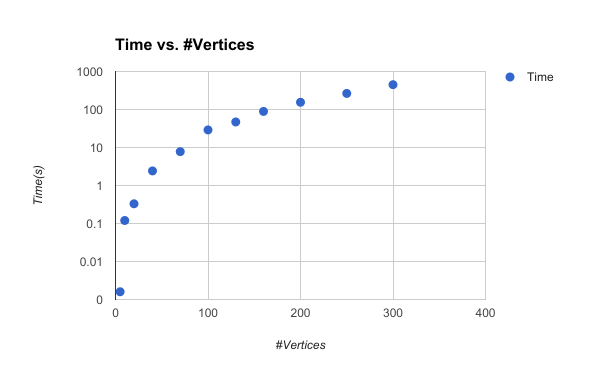
\epsfig{file=time.png,width=0.6\textwidth}
\end{center}
\end{figure}

\section*{Discussions}
For multi-path multi-commodity flow problem, solving the linear programming with a solver is fast enough for graphs with hundreds of vertices and edges. If only one path is allowed, it would request more integer constraints in linear programming and the performance is questionable. Our heuristic algorithm uses min-cost flow as subroutine to find a feasible solution for a pair of request, we could directly use shortest path instead to meet the single-path requirement. However, this won't work for the fast approximation algorithm for multi-commodity flow problem, since in this algorithm, the solution $x$ is a linear combination of multiple solutions. 

In our implementation heuristic algorithm, the amount penalty factor increment for a congested edge  is a fixed small number. This makes the updates slow, but the cost smaller. We may be able to dynamically adjust the amount for better timing and cost balance.

\bibliographystyle{alpha}
\bibliography{m-flow.bib}

\end{document}